
%\documentclass[mathserif]{beamer}
\documentclass[handout]{beamer}
%\usetheme{Goettingen}
%\usetheme{Warsaw}
\usetheme{Singapore}



%\usetheme{Frankfurt}
%\usetheme{Copenhagen}
%\usetheme{Szeged}
%\usetheme{Montpellier}
%\usetheme{CambridgeUS}
%\usecolortheme{}
%\setbeamercovered{transparent}
\usepackage[english, activeacute]{babel}
\usepackage[utf8]{inputenc}
\usepackage{amsmath, amssymb}
\usepackage{dsfont}
\usepackage{graphics}
\usepackage{cases}
\usepackage{graphicx}
\usepackage{pgf}
\usepackage{epsfig}
\usepackage{amssymb}
\usepackage{multirow}	
\usepackage{amstext}
\usepackage[ruled,vlined,lined]{algorithm2e}
\usepackage{amsmath}
\usepackage{epic}
\usepackage{epsfig}
\usepackage{fontenc}
\usepackage{framed,color}
\usepackage{palatino, url, multicol}
%\algsetup{indent=2em}
\newcommand{\factorial}{\ensuremath{\mbox{\sc Factorial}}}
\newcommand{\BIGOP}[1]{\mathop{\mathchoice%
{\raise-0.22em\hbox{\huge $#1$}}%
{\raise-0.05em\hbox{\Large $#1$}}{\hbox{\large $#1$}}{#1}}}
\newcommand{\bigtimes}{\BIGOP{\times}}
\vspace{-0.5cm}
\title{Natural Language Processing \\ Neural Networks}
\vspace{-0.5cm}
\author[Felipe Bravo Márquez]{\footnotesize
%\author{\footnotesize  
 \textcolor[rgb]{0.00,0.00,1.00}{Felipe Bravo-Marquez}} 
  
 

\date{\today}

\begin{document}
\begin{frame}
\titlepage


\end{frame}





\begin{frame}{Introduction to Neural Networks}
\begin{scriptsize}
\begin{itemize}
\item Very popular machine learning models formed by units called \textbf{neurons}.
\item A neuron is a computational unit that has scalar inputs and outputs. 
\item  Each input has an associated weight $w$.
 \item The neuron multiplies each input by its weight, and then sums them (other functions such as \textbf{max} are also possible). 
\item It applies an activation function $g$ (usually non-linear) to the result, and passes it to its output.
\item Multiple layers can be stacked.
\end{itemize}


\end{scriptsize}
\end{frame}


\begin{frame}{Activation Functions}

\begin{scriptsize}
\begin{itemize}
\item The nonlinear activation function $g$ has a crucial role in the network's ability to represent complex functions. 
\item Without the nonlinearity in g, the neural network can only represent linear transformations of the input.
\end{itemize}


\end{scriptsize}


\end{frame}


\begin{frame}{Feedforward Network with two Layers}


\begin{figure}[htb]
	\centering
	 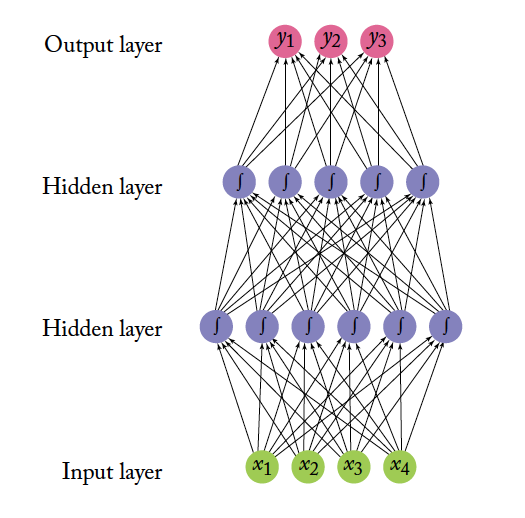
\includegraphics[scale=0.38]{pics/NN-example.png}
\end{figure}

\footnotetext{Source:\cite{goldberg2017neural}}

\end{frame}



\begin{frame}{Feedforward Network Neural Networks}
\begin{scriptsize}
\begin{itemize}
\item The feedforward network from the picture is a stack of linear models separated by nonlinear functions.
\item The values of each row of neurons in the network can be thought of as a vector. 

\item The input layer is a 4-dimensional vector $(\vec{x})$, and the layer above it is a 6-dimensional vector $(\vec{h}^1)$.
\item The fully connected layer can be thought of as a linear transformation from 4 dimensions to 6 dimensions. 
\item A fully connected layer implements a vector-matrix multiplication, $\vec{h}=\vec{x}W$.
\item The weight of the connection from the $i$-th neuron in the input row to the $j$-th neuron in the output row is $W_{[i,j]}$.
\item The values of $\vec{h}$ are transformed by a nonlinear function $g$ that is applied to each value before being passed on as input to the next layer.

\end{itemize}

\footnotetext{Vectors are assumed to be row vectors and superscript indices correspond to network layers.}

\end{scriptsize}
\end{frame}


\begin{frame}{Neural Netoworks as Mathematical Functions}
\begin{scriptsize}
\begin{itemize}
\item The Multilayer Perceptron (MLP) from the figure is called MLP2 because it has two hidden layers.
\item A simpler model would be MLP1, a multilayer perceptron of one hidden layer:
\begin{center}
\begin{equation}
\begin{split}
NN_{MLP1}(\vec{x}) = g(\vec{x}W^{1}+\vec{b}^{1})W^{2}+\vec{b}^{2} \\
\vec{x} \in \mathcal{R}^{in}, W^{1} \in \mathcal{R}^{d_{in}\times d_{1}}, \vec{b}^{1} \in \mathcal{R}^{1}, W^{1} \in \mathcal{R}^{in}, \vec{b}^{1} \in \mathcal{R}^{in}   
\end{split}
\end{equation}
\end{center}

\item Here $W^{1}$ and $\vec{b}^{1}$ are a matrix and a bias term for the first linear transformation of the input.
\item The function $g$ is a nonlinear function that is applied element-wise (also called a nonlinearity or an activation function ).
\item $W^{2}$ and $\vec{b}^{2}$ are the matrix and bias term for a second linear transform.

\item When describing a neural network, one should specify the dimensions of the layers ($d_{1}$) and the input ($d_{in}$).
\end{itemize}


\end{scriptsize}
\end{frame}




\begin{frame}{Neural Netoworks as Mathematical Functions}
\begin{scriptsize}
\begin{itemize}
\item MLP2 can be written as the following mathematical function:
\begin{center}
\begin{equation}
\begin{split}
NN_{MLP2}(\vec{x}) & =  \vec{y}  \\
\vec{h}^{1} &  = g^{1}(\vec{x}W^{1}+\vec{b}^{1}) \\
\vec{h}^{2} &  = g^{2}(\vec{h}^{1}W^{2}+\vec{b}^{2}) \\
\vec{y} &  = \vec{h}^{2}W^{3}\\
\vec{y} &  = (g^2(g^1(\vec{x}W^{1}+\vec{b}^{1})W^2+\vec{b}^2))W^3.\\
\end{split}
\end{equation}
\end{center}
\item The matrices and the bias terms that define the linear transformations are the parameters of the network. 
\item Like in linear models, it is common to refer to the collection of all parameters as $\Theta$.
\end{itemize}
\end{scriptsize}
\end{frame}



\begin{frame}{Representation Power}
\begin{scriptsize}
\begin{itemize}
\item \cite{hornik1989multilayer} and \cite{cybenko1989approximation} showed that a multilayer perceptron of one hidden later (MLP1) is a universal approximator.
\item MLP1 can approximate all continuous functions on a closed and bounded subset of $\mathcal{R}^n$.
\item This may suggest there is no reason to go beyond MLP1 to more complex architectures.
\item The result does not say how easy or hard it is to set the parameters based on training data and a specific learning algorithm.
\item It also does not guarantee that a training algorithm will find
the correct function generating our training data.
\item Finally, it does not state how large the hidden layer should be.
\end{itemize}


\end{scriptsize}
\end{frame}



\begin{frame}{Representation Power}
\begin{scriptsize}
\begin{itemize}
\item In practice, we train neural networks on relatively small amounts of data using local search methods.
\item We also use hidden layers of relatively modest sizes (up to several thousands). 
\item The universal approximation theorem does not give any guarantees under these conditions.
\item However, there is definitely benefit in trying out more complex architectures than MLP1. 
\item In many cases, however, MLP1 does indeed provide strong results.
\end{itemize}


\end{scriptsize}
\end{frame}








\begin{frame}{Activation Functions}
\begin{scriptsize}
\begin{itemize}
\item The nonlinearity $g$ can take many forms. 
\item There is currently no good theory as to which nonlinearity to apply in which conditions.
\item Choosing the correct nonlinearity for a given task is for the most part an empirical question.
\end{itemize}
\end{scriptsize}
\end{frame}


\begin{frame}{Sigmoid}
\begin{scriptsize}
\begin{itemize}
\item The sigmoid activation function $\sigma(x) = \frac{1}{1+e^{-x}}$ is an S-shaped function, transforming each value x into the range $[0, 1]$.
\item The sigmoid was the canonical nonlinearity for neural networks since their inception.
\item Is currently considered to be deprecated for use in internal layers of neural networks, as the choices listed next prove to work much better empirically.
\end{itemize}

\begin{figure}[htb]
	\centering
	 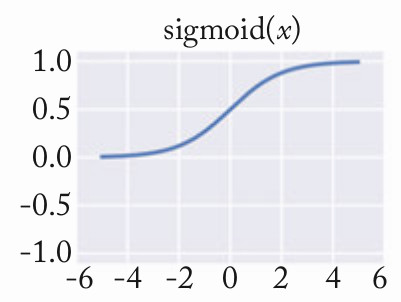
\includegraphics[scale=0.3]{pics/sigmoid2.png}
\end{figure}

\end{scriptsize}
\end{frame}



\begin{frame}{Hyperbolic tangent (tanh)}
\begin{scriptsize}
\begin{itemize}
\item The hyperbolic tangent $\operatorname{tanh}(x) = \frac{e^{2x}-1}{e^{2x}+1}$ activation function is an S-shaped function, transforming the values x into the range$[-1, 1]$.
\end{itemize}

\begin{figure}[htb]
	\centering
	 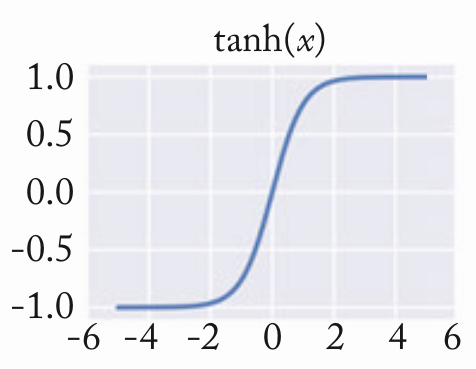
\includegraphics[scale=0.3]{pics/tanh.png}
\end{figure}

\end{scriptsize}
\end{frame}




\begin{frame}{Hard tanh}
\begin{scriptsize}
\begin{itemize}
\item The hard-tanh activation function is an approximation of the tanh function which is faster to compute and to find derivatives thereof:
\end{itemize}

  \[
    \operatorname{hardtanh}(x) = \left\{\begin{array}{lr}
        -1 & x < -1\\
        1 & x > 1\\
        x & \text{otherwise.} 
        \end{array} \right\} 
  \]

\begin{figure}[htb]
	\centering
	 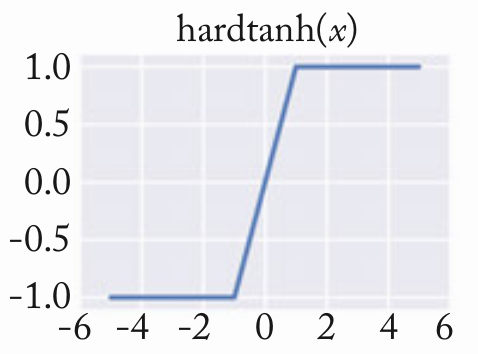
\includegraphics[scale=0.3]{pics/hardtanh.png}
\end{figure}

\end{scriptsize}
\end{frame}



\begin{frame}{ReLU}
\begin{scriptsize}
\begin{itemize}
\item The rectifier activation function \cite{glorot2011deep}, also known as the recti fied linear unit is a very simple activation function.
\item It is easy to work with and was shown many times to produce excellent results.
\item The ReLU unit clips each value $x < 0$ at $0$.
\begin{displaymath}
 \operatorname{ReLU}(x) = \operatorname{max}(0,x)
\end{displaymath}
\begin{figure}[htb]
	\centering
	 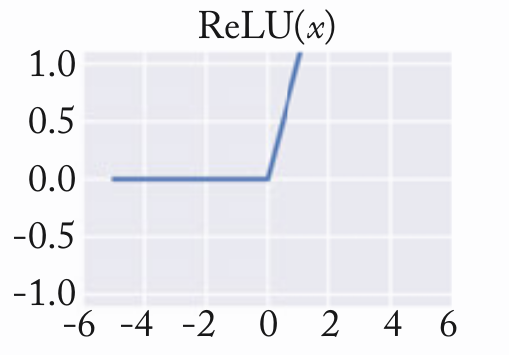
\includegraphics[scale=0.3]{pics/relu.png}
\end{figure}
\item It performs well for many tasks, especially when combined with the dropout regularization technique (to be explained later).
\end{itemize}
\end{scriptsize}
\end{frame}



\begin{frame}{Activation Functions}
\begin{scriptsize}
\begin{itemize}
\item As a rule of thumb, both ReLU and tanh units work well, and significantly outperform the sigmoid.
\item You may want to experiment with both tanh and ReLU activations, as each one may perform better in different settings.
\item The figure from below shows the shapes of the different activations functions, together with the shapes of their derivatives.
\end{itemize}
\begin{figure}[htb]
	\centering
	 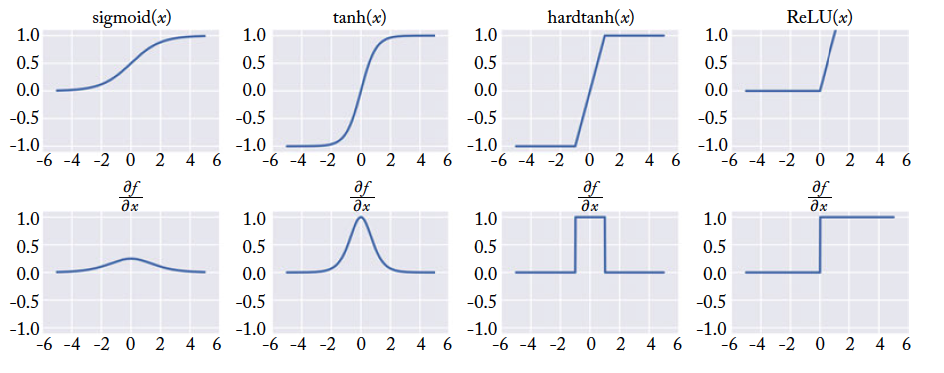
\includegraphics[scale=0.35]{pics/activations.png}
\end{figure}

\footnotetext{Source:\cite{goldberg2017neural}}
\end{scriptsize}
\end{frame}





\begin{frame}{Training}
\begin{scriptsize}
\begin{itemize}
\item  When training a parameterized function (e.g., a linear model, a neural network) one defines a loss function $L(\hat{y}, y)$, stating the loss of predicting $\hat{y}$ when the true output is y.

\item The training objective is then to minimize the loss across the different training examples. 

\item Functions are trained using  gradient-based methods.

\item They work by repeatedly computing an estimate of the loss $L$ over the training set.

\item They compute gradients of the parameters with respect to the loss estimate, and moving the parameters in the opposite directions of the gradient. 

\item Different optimization methods differ in how the error estimate is computed, and how moving in the opposite direction of the gradient is defined.

\end{itemize}


\end{scriptsize}
\end{frame}



\begin{frame}{Gradient Descent}
\begin{figure}[htb]
	\centering
	 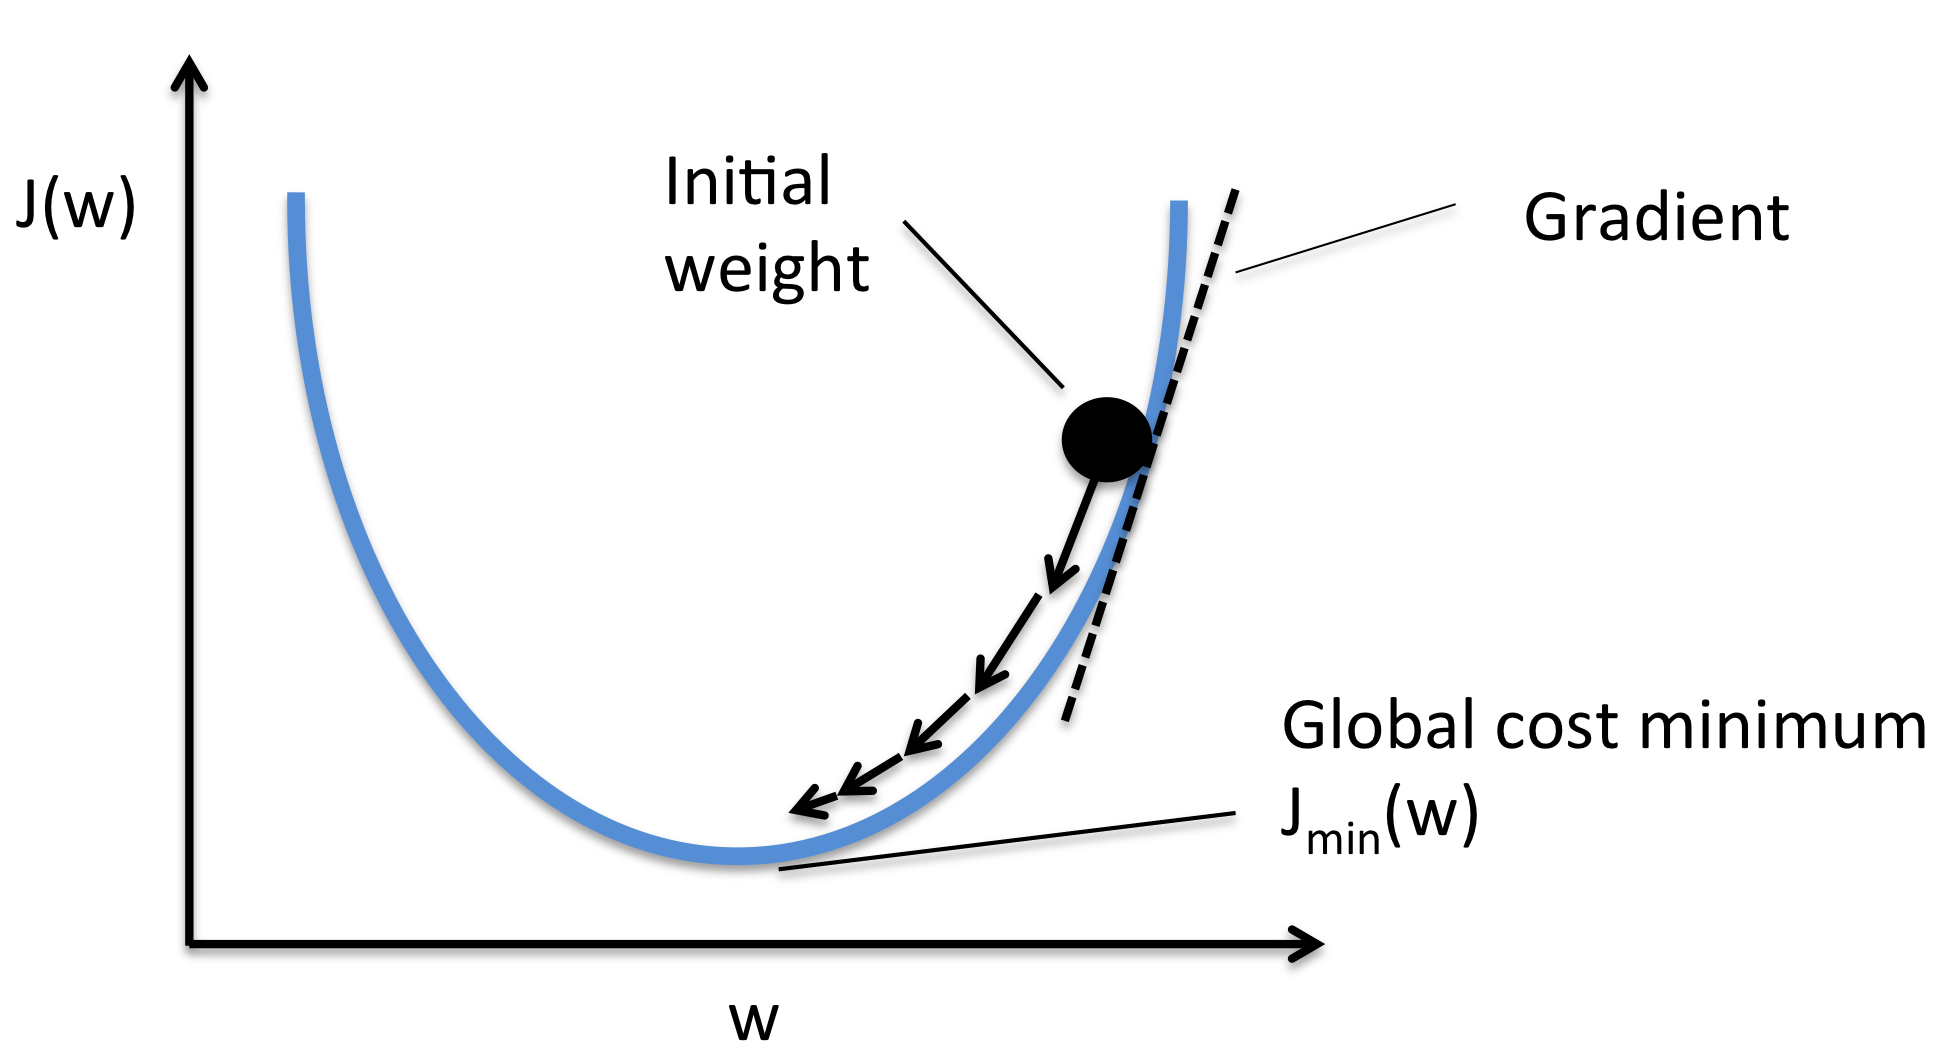
\includegraphics[scale=0.15]{pics/sgd.png}
\end{figure}

\footnotetext{Source: \url{https://sebastianraschka.com/images/faq/closed-form-vs-gd/ball.png}}

\end{frame}


\begin{frame}{Gradient Descent}
\begin{figure}[htb]
	\centering
	 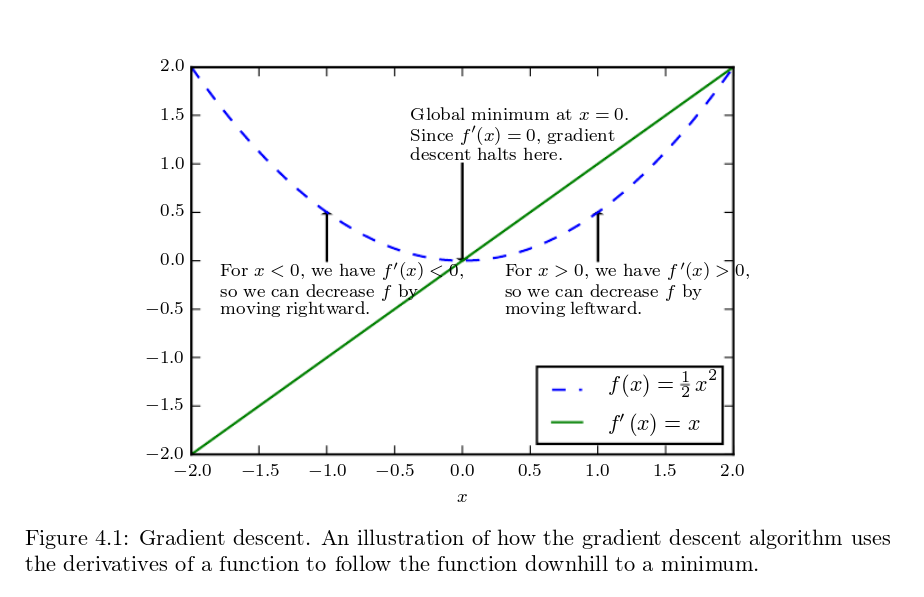
\includegraphics[scale=0.45]{pics/gradientdescent.png}
\end{figure}

\footnotetext{\cite{goodfellow2016deep}}

\end{frame}


\begin{frame}{Online Stochastic Gradient Descent}


\begin{figure}[htb]
	\centering
	 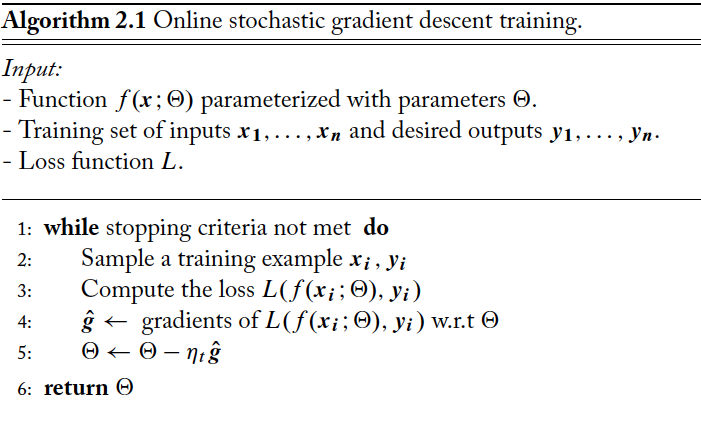
\includegraphics[scale=0.3]{pics/Online-SGD.png}
\end{figure}

\begin{scriptsize}
\begin{itemize}
\item The learning rate can either be fixed throughout the
training process, or decay as a function of the time step $t$.
\item  The error calculated in line 3 is based on a single training example, and is thus just a rough estimate of the corpus-wide loss $L$ that we are aiming to minimize. 
\item The noise in the loss computation may result in inaccurate gradients (single examples may provide noisy information).

\end{itemize}


\end{scriptsize}

\footnotetext{Source:\cite{goldberg2017neural}}

\end{frame}


\begin{frame}{Mini-batch Stochastic Gradient Descent}


\begin{scriptsize}
\begin{itemize}
\item A common way of reducing this noise is
to estimate the error and the gradients based on a sample of $m$ examples.
\item This gives rise to the minibatch SGD algorithm




\begin{figure}[htb]
	\centering
	 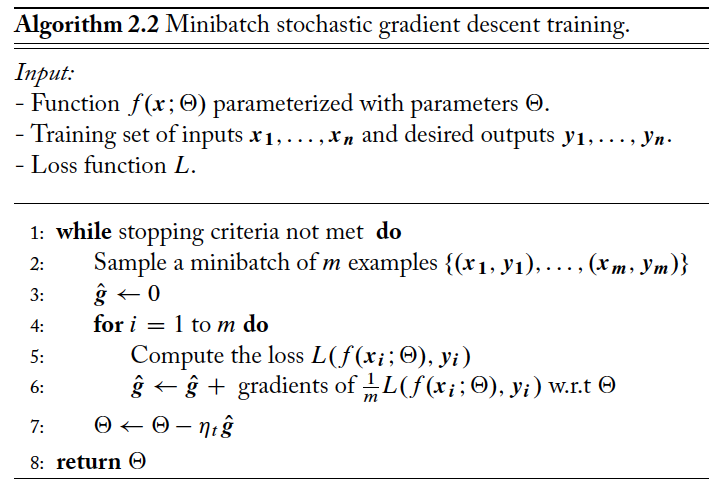
\includegraphics[scale=0.25]{pics/minibatch-SGD.png}
\end{figure}

\item Higher values of $m$ provide better estimates of the corpus-wide gradients, while smaller values allow more updates and in turn faster convergence.

\item For modest sizes of $m$ , some computing architectures (i.e., GPUs) allow an efficient parallel implementation of the computation in lines 3-6.

\end{itemize}
\end{scriptsize}

\footnotetext{Source:\cite{goldberg2017neural}}

\end{frame}



\begin{frame}{Loss Functions}
\begin{scriptsize}
\begin{itemize}
 \item Hinge (or SVM loss):  for binary classification problems, the classifier's output is a single scalar $\tilde{y}$ and the intended output y is in $\{+1,-1\}$.  The classification rule is $\hat{y} = sign(\tilde{y})$, and a classification is considered correct if $y \cdot \tilde{y} > 0$.  
 \begin{displaymath}
  L_{\text{hinge}(\text{binary})}(\tilde{y},y) = \max(0,1-y \cdot \tilde{y})  
 \end{displaymath}

 \item Binary cross entropy (or logistic loss): is used in binary classification with conditional probability outputs. The classifier's output $\tilde{y}$ is transformed using the sigmoid function to the range $[0,1]$ , and is interpreted as the conditional probability $P(y=1|x)$.
  \begin{displaymath}
  L_{\text{logistic}}(\hat{y},y) = -y \log \hat{y} - (1-y) \log(1-\hat{y})  
 \end{displaymath}
 
\end{itemize}
\end{scriptsize}

\end{frame}





\begin{frame}{Loss Functions}
\begin{scriptsize}
\begin{itemize}

 \item Categorical cross-entropy loss:  is used when a probabilistic interpretation of multi-class scores is desired. It measures the dissimilarity between the true label distribution $y$ and the predicted label distribution $\tilde{y}$. 
   \begin{displaymath}
  L_{\text{cross-entropy}}(\hat{y},y) = - \sum_{i} y_{[i]} \log(\hat{y}_{[i]})   
 \end{displaymath}
\item The predicted label distribution of the categorical cross-entropy loss ($\hat{y}$) is obtained by applying the softmax function the last layer of the network $\tilde{y}$:
    \begin{displaymath}
\hat{y}_{[i]} = \text{softmax}(\tilde{y})_{[i]} =  \frac{e^{\tilde{y}_{[i]}}}{\sum_{j}e^{\tilde{y}_{[j]}}}   
 \end{displaymath}
 
\item The softmax function squashes the $k$-dimensional output to values in the range (0,1) with all entries adding up to 1. Hence, $\hat{y}_{[i]} = P( y = i |x)$ represent the class membership conditional distribution.
 
\end{itemize}
\end{scriptsize}


\end{frame}




\begin{frame}{Backpropagation}
\begin{scriptsize}


\begin{itemize}
\item Backpropagation is an efficient technique for evaluating the gradient
of a loss function $L$ for a feed-forward neural network with respect to all its parameters \cite{bishop2006pattern}. \footnote{The following slides on backpropagation are based on \cite{bishop2006pattern}, we adapted the notation to be consistent with \cite{goldberg2017neural}.}
\item Those parameters are: $W^1, \vec{b}^1, \dots, W^m, \vec{b}^m$, for a network of $m$ layers.
\item Recall that superscripts are used to denote layer indexes (not exponentiations).
\item For simplicity, we will assume that $L$ is calculated over a single example.

\item In a general feed-forward network, each unit computes a weighted sum of its inputs in the form:
\begin{equation}
\vec{h}_{[j]}^l = \left(\sum_{i}  W_{[i,j]}^l \times \vec{z}_{[i]}^{(l-1)}\right) + \vec{b}_{[j]}^l 
\label{eq:sum}
\end{equation}

\item The variable $\vec{z}_{[i]}^{(l-1)}$ is an input that sends a connection to unit $\vec{h}_{[j]}^l$, $W_{[i,j]}^l$ is the weight associated with that connection, and $l$ is the layer index.

\item The biases vectors  $\vec{b}_{[j]}$ can be excluded from (eq.\ref{eq:sum}) and included to the weight matrix $W_{[i,j]}^l$ by introducing an extra unit, or input, with activation fixed at +1.

\end{itemize}


\end{scriptsize}
\end{frame}


\begin{frame}{Backpropagation}
\begin{scriptsize}


\begin{itemize}

\item The inputs at layer $l$, $\vec{z}_{[i]}^{(l-1)}$ are the result of applying the activation function $g$ to units from the previous layer:

\begin{equation}
\vec{z}_{[j]}^{l} = g(\vec{h}_{[j]}^{l})
\label{eq:ac}
\end{equation}

\item For the input layer ($l=0$), $\vec{z}$ corresponds to the input vector $\vec{z} = \vec{x}$ 

\begin{equation}
\vec{z}_{[j]}^0 = \vec{x}_{[j]}
\end{equation}

\item For each instance in the training set, we supply the corresponding input vector $\vec{x}$ to the network.
\item Next we calculate the activations of all of the hidden and output units in the network by successive application of (eq.\ref{eq:sum}) and (eq.\ref{eq:ac}). 

\item This process is often called forward propagation because it can be regarded
as a forward flow of information through the network.

\end{itemize}


\end{scriptsize}
\end{frame}


\begin{frame}{Backpropagation}
\begin{scriptsize}


\begin{itemize}

\item Now consider the evaluation of the derivative of $L$ with respect to a weight
$W_{[i,j]}^l$.

\item Assuming that the loss $L$ is calculated over a single example, we can note that $L$ depends on the weight $W_{[i,j]}^l$ only via the summed input $\vec{h}_{[j]}^{l}$.


\item We can therefore apply the chain rule for partial derivatives to give

\begin{equation}
\frac{\partial L}{\partial W_{[i,j]}^l} = \frac{\partial L}{\partial \vec{h}_{[j]}^{l}} \times \frac{\partial \vec{h}_{[j]}^{l}}{\partial W_{[i,j]}^l}
\label{eq:chain}
\end{equation}

\end{itemize}


\end{scriptsize}
\end{frame}



\begin{frame}{Backpropagation}
\begin{scriptsize}


\begin{itemize}


\item We now introduce a useful notation:

\begin{equation}
\vec{\delta}_{[j]}^l \equiv \frac{\partial L}{\partial \vec{h}_{[j]}^l}
\label{eq:delta}
\end{equation}

\item Using (\ref{eq:sum}), we can write
\begin{equation}
\frac{\partial \vec{h}_{[j]}^l}{\partial W_{[i,j]}^l} = \vec{z}_{[i]}^{(l-1)}
\label{eq:part}
\end{equation}

\item Substituting (\ref{eq:delta}) and (\ref{eq:part})  into (\ref{eq:chain}), we then obtain

\begin{equation}
\frac{\partial L}{\partial W_{[i,j]}^l} = \vec{\delta}_{[j]}^l \times \vec{z}_{[i]}^{(l-1)}
\label{eq:deltarule}
\end{equation}

\end{itemize}


\end{scriptsize}
\end{frame}


\begin{frame}{Backpropagation}
\begin{scriptsize}

\begin{itemize}
 \item  Equation (\ref{eq:deltarule}) tells us that the required derivative is obtained simply by multiplying the value of $\vec{\delta}_{[j]}^l$ by the value of $\vec{z}_{[i]}^{(l-1)}$.
 
 \item Thus, in order to evaluate the derivatives, we need only to calculate the value of $\vec{\delta}_{[j]}^l$ for each hidden and output unit in the network, and then apply (\ref{eq:deltarule}).
 
 \item Calculating $\vec{\delta}_{[j]}^m$ for output units ($l=m$), is usually straightforward, since activation units $\vec{h}_{[j]}^m$ are directly observed in the loss expression.
 
 \item The same applies for shallow linear models.
\end{itemize} 
\end{scriptsize}
\end{frame}


\begin{frame}{Backpropagation}
\begin{scriptsize}

\begin{itemize}
 \item To evaluate the $\vec{\delta}_{[j]}^l$ for hidden units, we again make use of the chain rule for partial derivatives:
 
 \begin{equation}
\vec{\delta}_{[j]}^l \equiv \frac{\partial L}{\partial \vec{h}_{[j]}^l} = \sum_{k}\left( \frac{\partial L}{\partial \vec{h}_{[k]}^{l+1}} \times \frac{\partial \vec{h}_{[k]}^{l+1}}{\partial \vec{h}_{[j]}^l}\right)
\label{eq:deltachain}
\end{equation}

\item The sum runs over all units $\vec{h}_{[k]}^{l+1}$ to which unit $\vec{h}_{[j]}^l$ sends connections.

\item We assume that connections go only to consecutive layers in the network (from layer $l$ to layer $(l+1)$).
\item The units $\vec{h}_{[k]}^{l+1}$  could include other hidden units and/or output units.

\item If we now substitute the definition of $\vec{\delta}_{[j]}^l$  given by (eq.\ref{eq:delta}) into (eq.\ref{eq:deltachain}), we get

 \begin{equation}
\vec{\delta}_{[j]}^l \equiv \frac{\partial L}{\partial \vec{h}_{[j]}^l} = \sum_{k}\left( \vec{\delta}_{[k]}^{(l+1)}  \times \frac{\partial \vec{h}_{[k]}^{l+1}}{\partial \vec{h}_{[j]}^l} \right)
\label{eq:delta2}
\end{equation}

\end{itemize}



\end{scriptsize}
\end{frame}



\begin{frame}{Backpropagation}
\begin{scriptsize}

\begin{itemize}
\item Now, for expression $\vec{h}_{[k]}^{l+1}$ we can go to its definition (eq.\ref{eq:sum}): 

\begin{displaymath}
\vec{h}_{[k]}^{(l+1)} = \left( \sum_{i} W_{[i,k]}^{l+1} \times \vec{z}_{[i]}^{l}\right) + \vec{b}_{[k]}^{(l+1)} 
\end{displaymath}

\item Now, we replace (eq.\ref{eq:ac}) $(\vec{z}_{[i]}^{l} = g(\vec{h}_{[i]}^{l}))$  
into previous equation and we obtain:

\begin{displaymath}
\vec{h}_{[k]}^{(l+1)} = \left( \sum_{i}   W_{[i,k]}^{l+1} \times g(\vec{h}_{[i]}^{l})\right)  + \vec{b}_{[k]}^{(l+1)}
\end{displaymath}


\item Now when calculating $\frac{\partial \vec{h}_{[k]}^{l+1}}{\partial \vec{h}_{[j]}^l}$ all the terms in the summation where $i \neq j$ get canceled out.   


\item Hence:

\begin{equation}
\frac{\partial \vec{h}_{[k]}^{l+1}}{\partial \vec{h}_{[j]}^l} =  W_{[j,k]}^{l+1} \times g'(\vec{h}_{[j]}^{l})
\label{eq:partialhh}
\end{equation}


\end{itemize}

\end{scriptsize}
\end{frame}


\begin{frame}{Backpropagation}
\begin{scriptsize}

\begin{itemize}
\item Now, if we substitute (eq.\ref{eq:partialhh}) into (eq.\ref{eq:delta2})


 \begin{equation}
\vec{\delta}_{[j]}^l \equiv \frac{\partial L}{\partial \vec{h}_{[j]}^l} = \sum_{k} \left( \vec{\delta}_{[k]}^{(l+1)}  \times W_{[j,k]}^{l+1} \times g'(\vec{h}_{[j]}^{l}) \right)
\label{eq:delta3}
\end{equation}

\item Since $g'(\vec{h}_{[j]}^{l})$ doesn't depend on $k$ we can obtain the following backpropagation formula:

 \begin{equation}
\vec{\delta}_{[j]}^l = g'(\vec{h}_{[j]}^{l}) \times \sum_{k} \left( \vec{\delta}_{[k]}^{(l+1)}  \times W_{[j,k]}^{l+1}\right)  
\label{eq:delta4}
\end{equation}

\item Which tells us that the value of $\delta$ for a particular hidden unit can be obtained by propagating the $\delta$'s backwards from units higher up in the network. \cite{bishop2006pattern}.

\end{itemize}

\end{scriptsize}
\end{frame}



\begin{frame}{Backpropagation }
\begin{scriptsize}
The backpropagation procedure can  be summarized as follows.
\begin{enumerate}
 \item Apply an input vector $\vec{x}$  to the network and forward propagate through
the network using (eq.\ref{eq:sum}) and (eq.\ref{eq:ac}) to find the activations of all the hidden and output units.
\item Evaluate the $\vec{\delta}_{[j]}^m$ for all the output units (recall that the derivatives involved here are easy to calculate).
\item Backpropagate the $\vec{\delta}_{[k]}^{(l+1)}$ using (eq.\ref{eq:delta4}) to obtain $\vec{\delta}_{[j]}^l$ for each hidden unit in the network. We go from higher to lower layers in the network.
\item Use (eq.\ref{eq:deltarule}) $(\frac{\partial L}{\partial W_{[i,j]}^l} = \vec{\delta}_{[j]}^l \times \vec{z}_{[i]}^{(l-1)})$ to evaluate the required derivatives.
\end{enumerate}


\end{scriptsize}
\end{frame}




\begin{frame}{The Computation Graph Abstraction}
\begin{scriptsize}
\begin{itemize}
\item  One can compute the gradients of the various parameters of a network by hand and implement them in code.

\item This procedure is cumbersome and error prone.

\item For most purposes, it is preferable to use automatic tools for gradient computation [Bengio, 2012].

\item A computation graph is a representation of an arbitrary mathematical computation (e.g., a neural network) as a graph.

\item Consider for example a graph for the computation of $(a*b+1)*(a*b+2)$:

\begin{figure}[htb]
	\centering
	 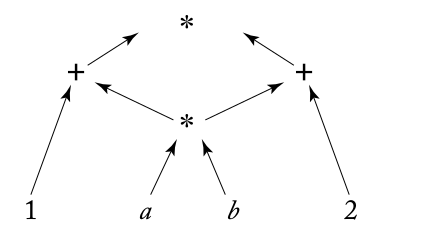
\includegraphics[scale=0.25]{pics/compGraph.png}
\end{figure}

\item The computation of $a*b$ is shared.

\item The graph structure defines the order of the computation in terms of the dependencies between the different components.

\end{itemize}
\end{scriptsize}
\end{frame}






\begin{frame}{The Computation Graph Abstraction}
\begin{scriptsize}
\begin{itemize}

\item  Te computation graph abstraction allows us to:


\begin{enumerate}
\begin{scriptsize}
 \item Easily construct arbitrary networks.
 \item Evaluate their predictions for given inputs (forward pass)
 
 \begin{figure}[htb]
	\centering
	 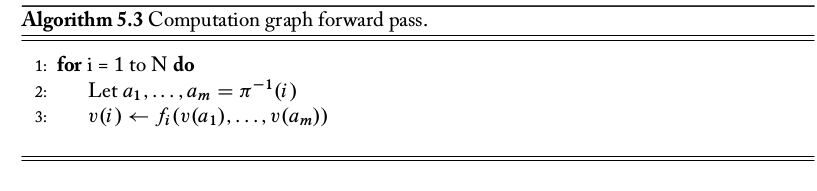
\includegraphics[scale=0.25]{pics/forwardPass.png}
\end{figure}

 
 
 \item Compute gradients for their parameters with respect to arbitrary scalar losses (backward pass or backpropagation).
 
 
  
 \begin{figure}[htb]
	\centering
	 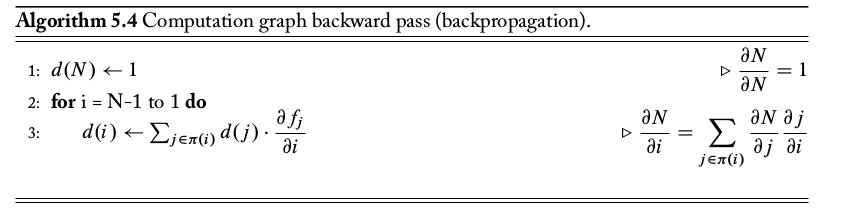
\includegraphics[scale=0.25]{pics/backwardPass.png}
\end{figure}
 
\end{scriptsize}
 \end{enumerate}
  
  
  
  
 \item The backpropagation algorithm (backward pass) is essentially following the chain-rule of differentiation\footnote{A comprehensive tutorial on the backpropagation algorithm over the computational graph abstraction: \url{https://colah.github.io/posts/2015-08-Backprop/}}.
 
  
\end{itemize}
\end{scriptsize}
\end{frame}






\begin{frame}{Train, Test, and Validation Sets}
\begin{scriptsize}
\begin{itemize}
\item Neural networks are prone to overfit the data.
\item Hence, performance on training data can be misleading.
\item Held-out set: split training set into training and testing subsets (80\% and 20\% splits). Train on training and compute accuracy on testing.
\item Problem: in practice you often train several models, compare their quality, and select the best one. 
\item Selecting the best model according to the held-out set's accuracy will result in an overly optimistic estimate of the model's quality.
\item You don't know if the chosen settings of the final classifier are good in general, or are just good for the particular examples in the held-out sets.

\end{itemize}
\end{scriptsize}
\end{frame}


\begin{frame}{Train, Test, and Validation Sets}
\begin{scriptsize}
\begin{itemize}
\item The accepted methodology is to use a three-way split of the data into train, validation (also called development ), and test sets \footnote{An alternative approach is cross-validation, but it doesn't scale well for training deep neural networks.}. 
\item This gives you two held-out sets: a validation set (also called development set ), and a test set.
\item All the experiments, tweaks, error analysis, and model selection should be performed based on the validation set. 
\item Then, a single run of the final model over the test set will give a good estimate of its expected quality on unseen examples. 
\item It is important to keep the test set as pristine as possible, running as few experiments as possible on it. 
\item Some even advocate that you should not even look at the examples in the test
set, so as to not bias the way you design your model.



\end{itemize}

\end{scriptsize}
\end{frame}



\begin{frame}{Train, Test, and Validation Sets}
\begin{scriptsize}

 \begin{figure}[htb]
	\centering
	 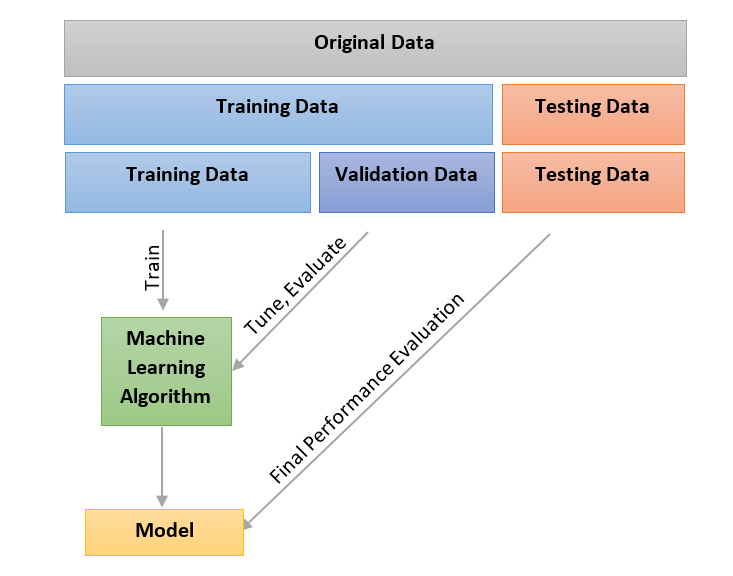
\includegraphics[scale=0.55]{pics/validation.png}
\end{figure}

\footnotetext{source: \url{https://www.codeproject.com/KB/AI/1146582/validation.PNG}}

\end{scriptsize}
\end{frame}



\begin{frame}{Deep Learning Frameworks}
Several software packages implement the computation-graph model. All these packages support all the essential components (node types) for defining a wide range of neural network architectures.
\begin{scriptsize}
\begin{itemize}
\item TensorFlow (\url{https://www.tensorflow.org/}): an open source software library for numerical computation using data-flow graphs originally developed by the Google Brain Team. 

\item Keras: High-level neural network API that runs on top of Tensorflow as well as other backends (\url{https://keras.io/}). 

\item PyTorch: open source machine learning library for Python, based on Torch, developed by Facebook's artificial-intelligence research group. It supports dynamic graph construction, a different computation graph is created from scratch for each training sample. (\url{https://pytorch.org/})


\end{itemize}
\end{scriptsize}
\end{frame}




\begin{frame}
\frametitle{Questions?}
%\vspace{1.5cm}
\begin{center}\LARGE Thanks for your Attention!\\ \end{center}



\end{frame}

\begin{frame}[allowframebreaks]\scriptsize
\frametitle{References}
\bibliography{bio}
\bibliographystyle{apalike}
%\bibliographystyle{flexbib}
\end{frame}  


%%%%%%%%%%%%%%%%%%%%%%%%%%%

\end{document}
